\chapter{Аналитический раздел}

В данном разделе проводится постановка задачи, цель разработки проекта, анализ предметной области, рассмотрение понятий и существующих методов нейронных сетей для решения задачи. Проводится обзор существующих методов, а также устанавливаются критерии сравнения и классификации этих методов.

\section{Постановка задачи}

Цель разработки программы является выявление и восстановление размытого изображения. Программа принимает на вход размытое изображение и выдаёт пользователю восстановленное изображение от размытия.

На рисунке (\ref{fig:method-desc}) представлено, формализация задачи восстановление размытие изображение: 
\begin{figure}[H]
	\centering
	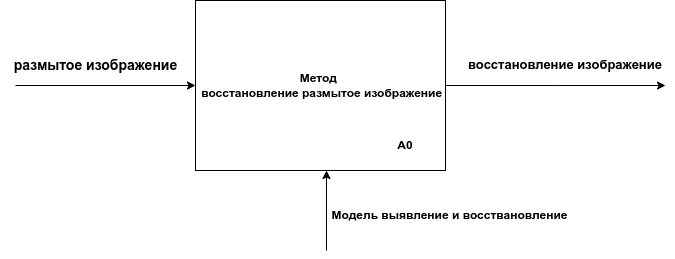
\includegraphics[width=1\linewidth]{assets/idef0.png}
	\caption{Формализация задачи восстановление размытие изображение}
	\label{fig:method-desc}
\end{figure}

\section{Анализ предметной области}

% В данной формулировке предполагается, что идеальное изображение \(x \in \mathbb{R}^{N}\) происходит из множества изображений, описываемого функцией плотности вероятности \(p(x)\). Измерением является вектор \(y \in \mathbb{R}^{N}\), определенный уравнением \cite{elad2023image}:

% \begin{equation}
%     y = x + v,
% \end{equation}

% где \(v \in \mathbb{R}^{N}\) представляет собой гауссовский шум с нулевым средним и одинаково распределенным, \(v \sim \mathcal{N}(0, \sigma^{2}I)\).

% Задача удаления шума заключается в восстановлении \(x\) из \(y\) при известном параметре \(\sigma\). Таким образом, шумоподавитель представляет собой функцию вида \(\hat{x} = D(y, \sigma)\) \cite{kong2023comparison}.

Размытие изображения может быть вызвано различными факторами во время съемки: дрожанием камеры, движением в кадре или размытием не в фокусе. размытое изображение \(I_{b}\) обозначают как:

\begin{equation}
	I_{b} = \phi(I_{s}; \theta_{\eta}),
\end{equation}


где \(\phi\) это функция размытия изображения, а \(\theta_{\eta}\) это вектор параметров. \(I_{s}\) это скрытая четкая версия размытого изображения \(I_{b}\). Методы устранения размытия можно разделить на незрячие и слепые методы \cite{zhang2022deep}, в зависимости от того, известна функция размытия или нет. Целью устранения размытия изображения является восстановление четкости изображения, т.е. нахождение обратной функции размытия, как:

\begin{equation}
	I_{db} = \phi^{-1}(I_{b}; \theta_{\eta}),
\end{equation}


где \(\phi^{-1}\) это модель устранения размытия и \(I_{db}\) обозначает размытое изображение, которое является оценкой скрытой резкости изображения.

В целом наличие размытия на изображении делиться на четырх категории:

\begin{itemize}
	\item Размытие в движении;
	\item Размытие вне фокуса;
	\item Размытие по Гауссу;
	\item Cмешанное размытие.
\end{itemize}

\subsection{Размытие в движении}

Изображение получается путем измерения фотонов за период времени воздействия камеры. При ярком освещении время экспозиции достаточно короткое, чтобы изображение смогло запечатлеть мгновенный момент. Однако более длительное время выдержки может привести к размытию изображения при движении. Многочисленные методы напрямую моделируют процесс деградации как процесс свертки, предполагая, что размытие равномерно по всему изображению \cite{gao2019dynamic}:

\begin{equation}
	I_{b} = K * I_{s} + \theta_{\mu},
\end{equation}

где \(K\) - ядро размытия, а \(\theta_{\mu}\) — аддитивный гауссов шум. На таком изображении любой объект, движущийся относительно камеры, будет выглядеть размытым в направлении относительного движения.

\subsection{Размытие вне фокуса}

Помимо размытия в движении, на резкость изображения также влияет расстояние между сценой и фокальной плоскостью камеры. Точки в фокальной плоскости находятся в истинном фокусе, а точки, расположенные рядом с ней, появляются в фокусе, определяя глубину резкости. Если сцена содержит объекты за пределами этой области, части сцены будут выглядеть размытыми \cite{zhang2020deblurring}. Функция распределения точек для размытия вне фокуса часто моделируется как:

\begin{equation}\label{eq:deblurring}
	K(x, y) = \begin{cases}
		\frac{1}{2 \pi r^2}, & \text{если } (x - k)^2 + (y - l)^2 \leq r^2, \\
		0, & \text{иначе},
	\end{cases}
\end{equation}

где \(k\) и \(l\) - центр функции распределения точек, а \(r\) - радиус размытия.

\subsection{Размытие по Гауссу}

Размытие по Гауссу - это распространенная простая модель размытия, используемая при обработке изображений, определяемая как \cite{chen2009empirical}:

\begin{equation}
	G(x, y) = \frac{1}{2 \pi \sigma^2} e^{-\frac{(x - k)^2 + (y - l)^2}{2 \sigma^2}},
\end{equation}

где \(x\) и \(y\) - расстояние от начала координат по горизонтальной и вертикальной оси соответственно, \(\sigma\) - стандартное отклонение.


\subsection{Смешанное размытие}

Во многих реальных сценах на размытие влияют различные факторы, такие как дрожание камеры, движение объекта и изменение глубины. Например, когда быстро движущийся объект снимается на расстоянии вне фокуса, изображение может включать как размытие в движении, так и размытие вне фокуса. Чтобы синтезировать этот тип размытого изображения, один из вариантов состоит в том, чтобы сначала преобразовать резкие изображения в их версии с размытием в движении, а затем применить ядро размытия вне фокуса на основе уравнения (\ref{eq:deblurring}) \cite{zhang2020deblurring}.


На рисунке (\ref{fig:blur-types}) представлено, примеры различных размытых изображений: 
\begin{figure}[H]
	\centering
	\includegraphics[width=1\linewidth]{assets/blur-types.png}
	\caption{Примеры различных размытых изображений}
	\label{fig:blur-types}
\end{figure}

В таблице (\ref{tab:blur_comparison}), проводится сравнение размытия изображения.

\begin{table}[H]
    \centering
    \caption{Сравнение размытия изображения}
    \label{tab:blur_comparison}
    \begin{tabular}{|p{3cm}|p{4cm}|p{4cm}|p{4cm}|}
        \hline
        \textbf{Категория размытия} & \textbf{Источник размытия} & \textbf{Математическая модель} & \textbf{Эффект на изображение} \\ \hline
        Размытие в движении & Движение объектов относительно камеры & Свертка с ядром размытия & Размытие объектов в направлении движения \\ \hline
        Размытие вне фокуса & Расстояние между сценой и фокусной плоскостью камеры & Функция распределения точек & Размытие объектов вне области фокуса \\ \hline
        Размытие по Гауссу & Математическая модель Гауссового распределения & Функция Гаусса & Мягкое, равномерное размытие вокруг объектов \\ \hline
        Смешанное размытие & Различные факторы, включая дрожание камеры, движение объекта, изменение глубины & Комбинация методов размытия в движении и вне фокуса & Синтез сложных эффектов размытия, характерных для реальных сцен \\ \hline
    \end{tabular}
\end{table}

\section{Нейроные сети}

Первоначальное развитие этих сетей берет свое начало в работе Фрэнка Розенблатта о персептронах и начинается с определения нейрона \cite{DOU2023484}. Математически нейрон - это нелинейность, применяемая к аффинной функции. Входные характеристики \(x = (x_1, x_2, . . . , x_n)\) передаются через аффинную функцию, составленную с нелинейностью \(\phi\):

\begin{equation}
    T(x) = \phi\left(\sum_{i} W_{i} \ast x_{i} + b\right) = \phi(W \ast x + b)
, \end{equation}

с заданными весами \(W\) и смещением \(b\). Схематично это представлено на рисунке (\ref{fig:neuron}). Типичной нелинейностью, или функцией активации, является сигмоидная форма, определяемая как:

\begin{equation}
    \phi(x) = \frac{1}{1 + e^{-x}}
, \end{equation}

Функция активации не обязательно должна быть только сигмоидной; она выбирается в зависимости от задачи, которую необходимо решить с использованием нейронных сетей.

На рисунке (\ref{fig:neuron}) представлено, cхематическая версия нейрона: 
\begin{figure}[H]
	\centering
	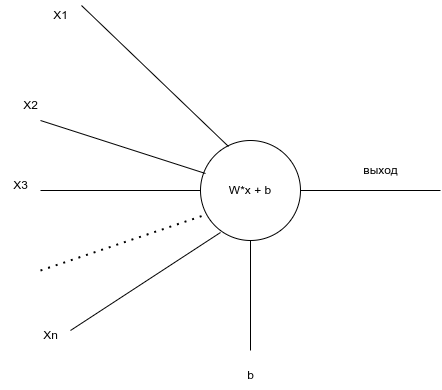
\includegraphics[width=0.5\linewidth]{assets/neuron.png}
	\caption{Схематическая версия нейрона}
	\label{fig:neuron}
\end{figure}

Нейронную сеть можно смоделировать как набор нейронов, которые соединены в ациклический граф. То есть выходные данные некоторых нейронов становятся входными данными для других нейронов, и циклы, в которых выходные данные нейрона отображаются обратно на более ранний промежуточный вход, запрещены. Обычно такие нейроны организованы в слои нейронов. Такая сеть состоит из входного слоя, одного или нескольких скрытых слоев и выходного слоя. В отличие от скрытых слоев, выходной слой обычно не имеет функции активации.

В зависимости от задачи нейронные сети могут обучаться контролируемым или неконтролируемым способом и соответствено в нейронных сетей появится термин функция потерь, также называемая функцией стоимости или целевой функцией, играет ключевую роль в измерении несоответствия между прогнозируемым выходным сигналом сети и фактическими целевыми значениями. Основная цель на этапе обучения — минимизировать эту функцию потерь, поскольку это повышает точность модели при составлении прогнозов и для того что бы уменьшить потери изпользуется обратное распространение ошибки и так представляется:

\begin{equation}
    \frac{\partial L}{\partial W} = \frac{\partial L}{\partial T} * \frac{\partial T}{\partial Z} * \frac{\partial Z}{\partial W}
, \end{equation}

Где \(\frac{\partial L}{\partial W}\) — это градиент функции потерь по весам W.

На рисунке (\ref{fig:neuron-arch}) представлено, трехслойная нейронная сеть с тремя входами и двумя скрытыми слоями: 
\begin{figure}[H]
	\centering
	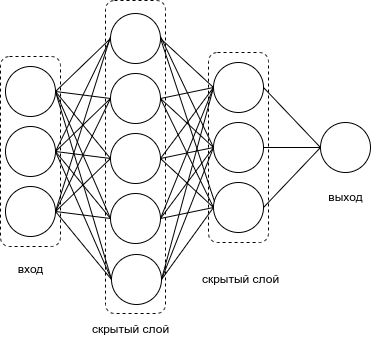
\includegraphics[width=0.5\linewidth]{assets/neural-arch.png}
	\caption{Трехслойная нейронная сеть с тремя входами и двумя скрытыми слоями}
	\label{fig:neuron-arch}
\end{figure}

\subsection{Сверточная нейронная сеть (CNN)}

Сверточные нейронные сети (CNN) представляют собой частный случай нейронных сетей с прямой связью. В отличие от обычных нейронных сетей, слои CNN содержат нейроны, расположенные в нескольких измерениях: в каналах, ширине, высоте и количестве фильтров в простейшем двумерном случае.

Наиболее распространенными строительными блоками, с которыми столкиваются в большинстве архитектур CNN, являются уровень свертки, уровень пула и полностью связанные уровни.

\subsection*{Cвертки}

Математическая свертка \((x * w)(a)\) функций \(x\) и \(w\) определяется во всех измерениях как:

\begin{equation}
    (x * w)(a) = \int x(t) * w (t - a) \, da
, \end{equation}

где \(a\) находится в \(R^{n}\) для любого \(n \ge 1\), а интеграл заменяется его многомерным вариантом. В терминологии сверточных нейронных сетей \(x\) называется входом, \(w\) называется фильтром или ядром, а выход часто называют активацией или картой признаков.

\subsubsection*{Нелинейности}

Нелинейности необходимы для проектирования нейронных сетей, без них нейронная сеть будет вычислять линейную функцию своих входных данных, что является слишком ограничительным. Выбор нелинейности может оказать большое влияние на скорость обучения нейронной сети. Следовательно, часто после того, как мы получаем результаты из каждой свертки, мы применяем функцию активации.

\subsubsection*{Объединение слоев}

Целью слоя объединения является создание сводной статистики его входных данных и уменьшение пространственных размеров карты объектов. Наиболее распространенной формой является максимальный пул, который использует шаг 2 вместе с размером ядра 2. Это соответствует пространственному разбиению карты объектов на регулярную сетку квадратных или кубических блоков со стороной 2 и взятию максимального или среднего значения по таким блокам для каждого входного объекта.

На рисунке (\ref{fig:max-pool}) представлено, максимальный пул c шагом 2 вместе с размером ядра 2: 
\begin{figure}[H]
	\centering
	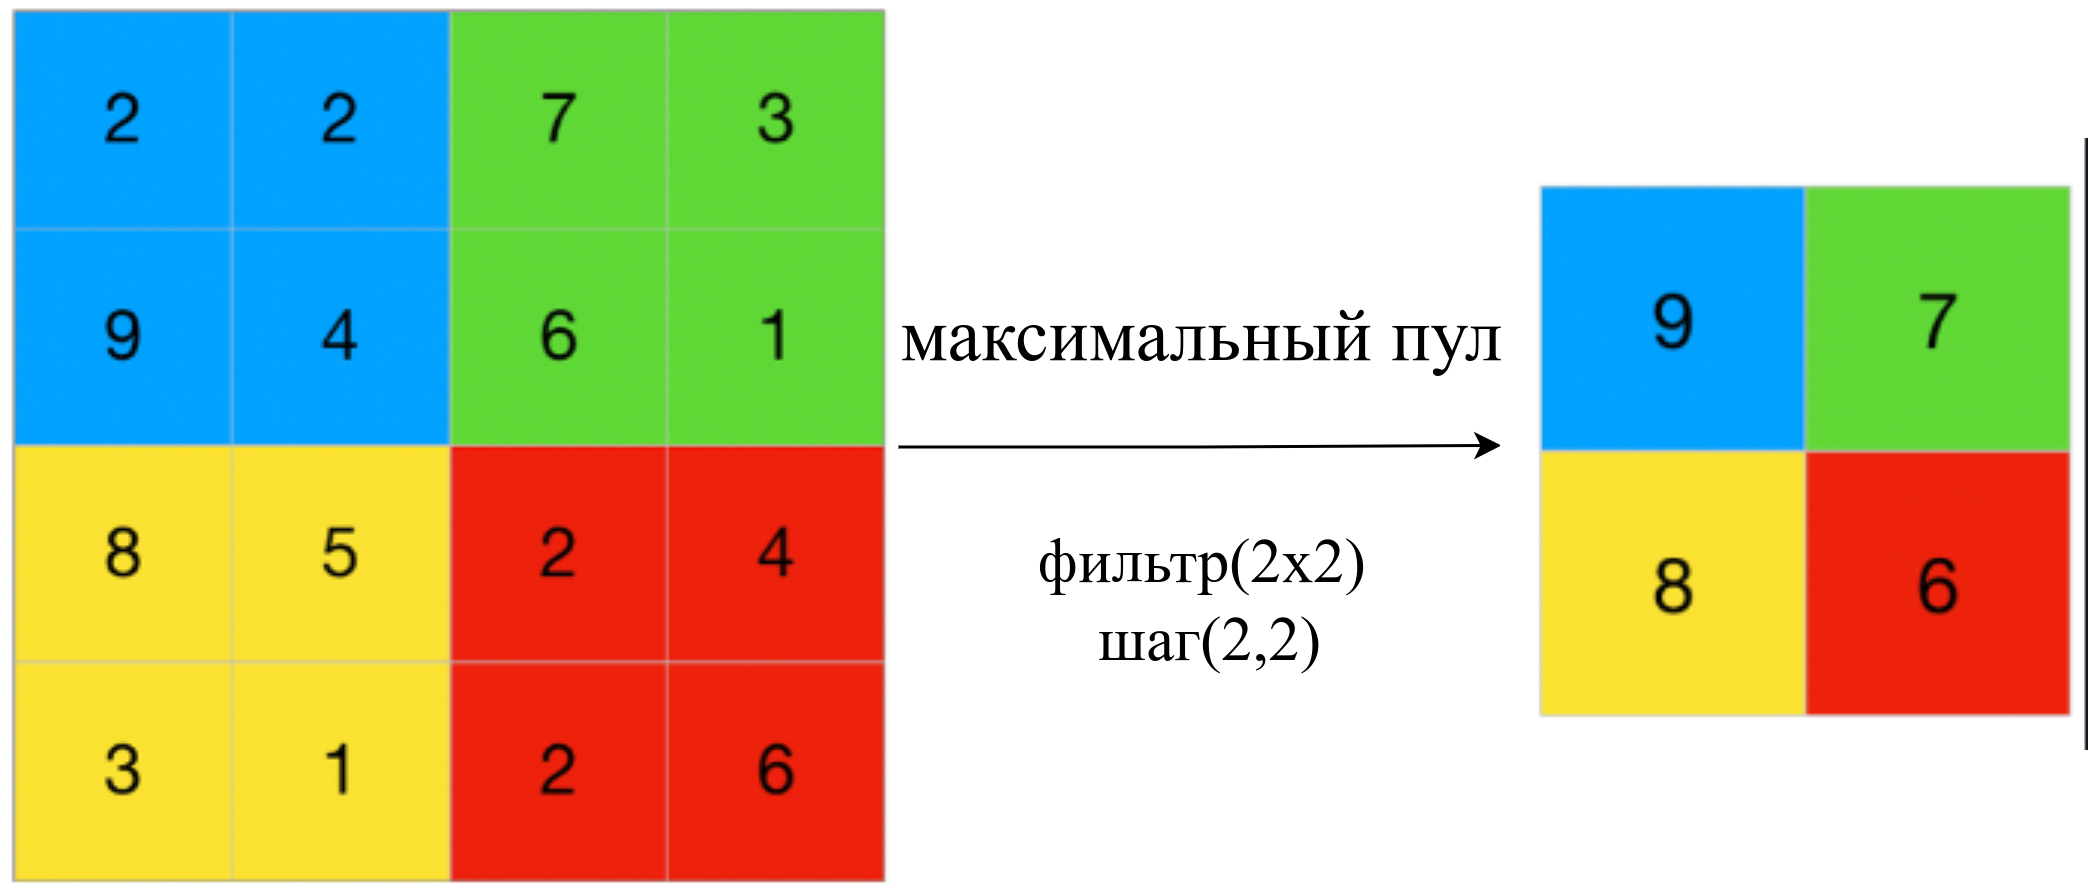
\includegraphics[width=0.5\linewidth]{assets/max-pooling.png}
	\caption{максимальный пул c шагом 2 вместе с размером ядра 2}
	\label{fig:max-pool}
\end{figure}

\subsubsection*{Полностью связанные слои}

Полностью связанный слой с \(n\) входными измерениями и \(m\) выходными измерениями определяется следующим образом.

Выход слоя определяется параметрами: весовой матрицей \(W \in \mathbb{M}_{m,n}(\mathbb{R})\), имеющей \(m\) строк и \(n\) столбцов, и вектором смещения \(b \in \mathbb{R}^{m}\). Для данного входного вектора \(x \in \mathbb{R}^{n}\), выход полносвязного слоя \(FC\) с функцией активации \(f\) определяется как:

\begin{equation}
    FC(x) := f(W \cdot x + b) \in \mathbb{R}^{m}
, \end{equation}

В приведенной выше формуле \(W \cdot x\) — это произведение матриц, а функция \(f\) применяется покомпонентно.

\subsection{Остаточная нейронная сеть (ResNet)}

Остаточные нейронные сети состоят из множества остаточных блоков \cite{he2016deep}. Учитывая остаточный блок \(l\) и его входные данные \(x\), выходные данные определяются как:

\begin{equation}
    x_{l + 1} = \sigma(F_{l}(x_{l}) + x_{l})
, \end{equation}

В формуле \(F_{l}\) обозначает остаточную функцию, где \(F_{l}(x) = \text{BN}(W_{l,2} \cdot \sigma(\text{BN}(W_{l,1} \cdot x)))\), а \(W_{l,1}\) и \(W_{l,2}\) являются сверточными весовыми матрицами, \(\text{BN}(x)\) обозначает пакетную нормализацию, а \(\sigma(x)\) - функцию активации.

На рисунке (\ref{fig:residual-block}) представлено, остаточный блок: 
\begin{figure}[H]
	\centering
	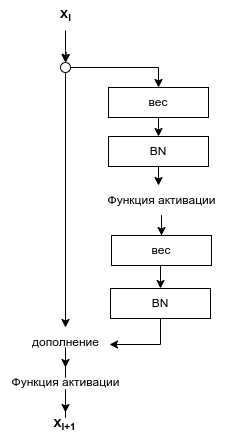
\includegraphics[width=0.3\linewidth]{assets/residual-block.png}
	\caption{Остаточный блок}
	\label{fig:residual-block}
\end{figure}

Однако данная формулировка трудно интерпретируется аналитически, и она не содержит "истинного" соединения с пропуском идентификации из-за конечного компонента функции активации. Вместо этого используется остаточный блок с предварительной активацией \cite{he2016identity}. Учитывая остаточный блок \(l\) и его входной сигнал \(x_{l}\), выходной сигнал теперь определяется как:

\begin{equation}
    x_{l + 1} = \sigma(F_{l}(x_{l}) + x_{l})
, \end{equation}

В формуле \(F_{l}\) обозначает остаточную функцию, где \(F_{l}(x) = W_{l,2} \cdot \text{BN}(\sigma(W_{l,1}) \cdot \sigma(\text{BN}(x)))\). Эта формулировка более четко выводится из интуиции, поскольку мы непосредственно добавляем выходные данные слоя к выходным данным следующего слоя.

Рекурсивно, пишется следующим образом:

\begin{equation}
    x_{l + 1} = x_{l} + \sum_{i = l}^{L - 1} F_{i}(x_{i})
, \end{equation}

для более глубокого остаточного блока \(L\) и более мелкого остаточного блока \(l\). Эта формулировка поддерживает путь идентификации по всей сети, поэтому теоретически, если более мелкие остаточные блоки сети способны идентифицировать разумное представление, сеть может обойти остальные уровни, используя пропускные соединения.

Мы также можем удалить все остаточные соединения, чтобы сформировать стандартную сеть, где, рассматривая пары сверточных слоев, мы получаем аналогичные уравнения:

\begin{equation}
    x_{l} = F_{l}(x_{l})
, \end{equation}

И таким образом, получим:

\begin{equation}
    x_{l} = F_{L - 1}(F_{L - 2}(\ldots F_{1}(x_{1})))
, \end{equation}

\subsection{Капсулные нейронные сети (CapsNet)}

Капсульные сети, предложенные в качестве альтернативы сверточным нейронным сетям, являются эквивариантными и состоят из сети нейронов, которая принимает и выводит векторы, в отличие от скалярных значений в CNN. Это свойство позволяет капсулам изучать особенности изображения в дополнение к его деформациям и условиям просмотра. В капсульной сети каждая капсула представляет собой группу нейронов, и выходные данные каждого нейрона представляют различные свойства одного объекта. Это обеспечивает преимущество в распознавании целого объекта путем предварительного распознавания его частей \cite{lecun2015deep}.

Входными данными для капсулы являются выходные данные CNN. Эти признаки обрабатываются в зависимости от типа используемой капсулы. Выходные данные капсулы включают в себя вероятность наличия признака, закодированного капсулой, и набор векторных значений, обычно называемых параметрами экземпляра. Вероятность наличия элемента капсулы отвечает за обеспечение инвариантности сети. Параметры экземпляра используются для представления эквивариантности сети, указывая на ее способность распознавать позу, текстуру и деформации. Инвариантность это свойство решения модели оставаться неизменным независимо от любых преобразований входных данных \cite{patrick2022capsule}.

На рисунке (\ref{fig:residual-block}) представлено, архитектура кусульных нейронных сетей: 
\begin{figure}[H]
	\centering
	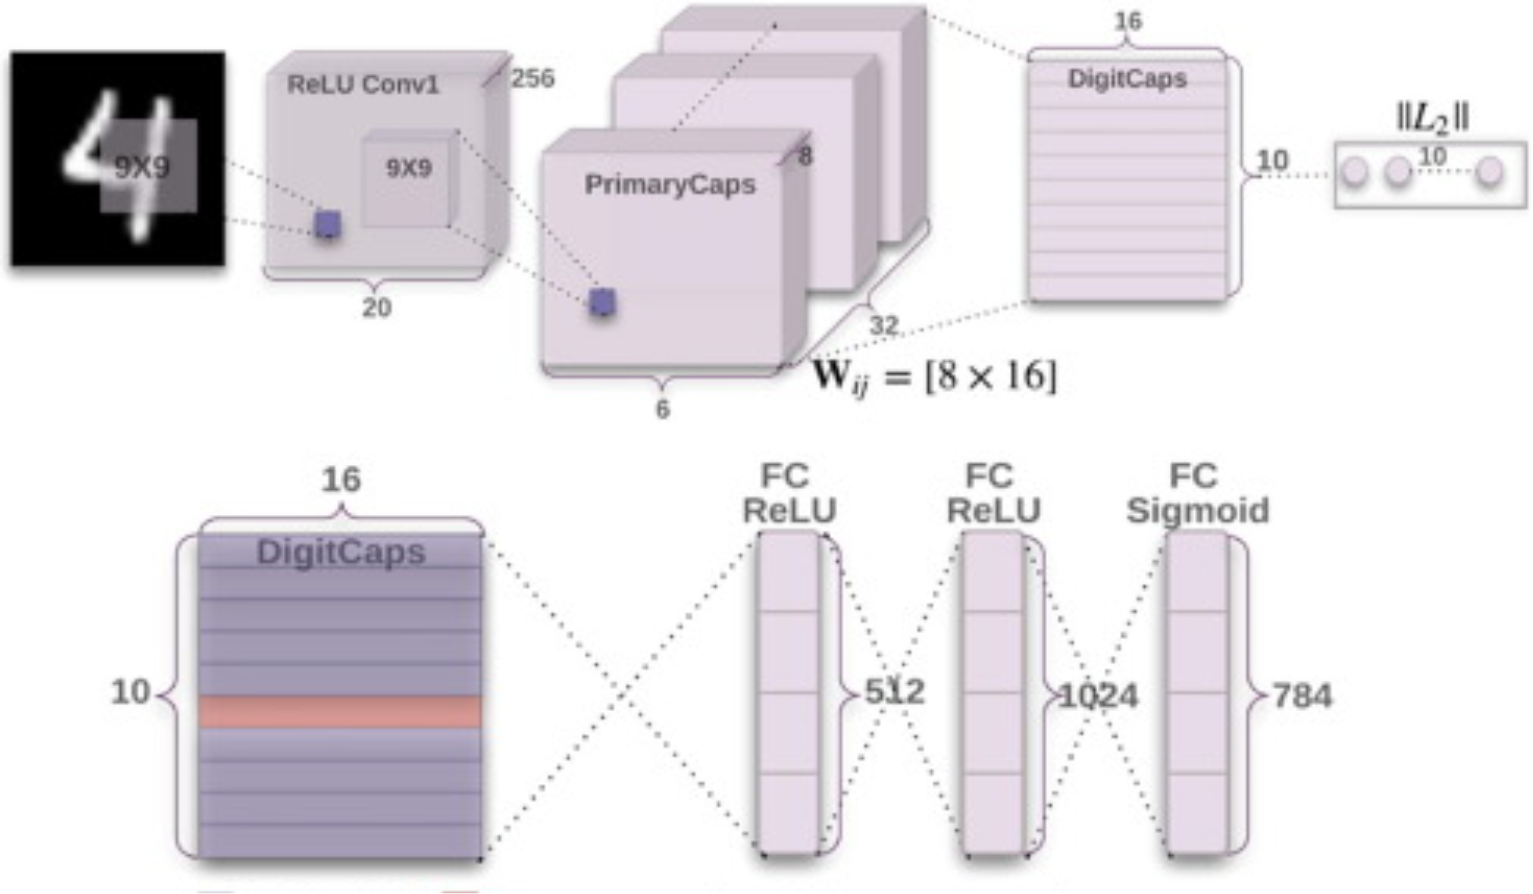
\includegraphics[width=0.6\linewidth]{assets/capsnet.png}
	\caption{Архитектура кусульных нейронных сетей}
	\label{fig:residual-block}
\end{figure}

Капсула \(i\) в капсульной сети может быть представлена в виде вектора \(v_{i}\), а выходной сигнал капсулы может быть представлен в виде нелинейной функции вектора:

\begin{equation}
    u_{i} = f(W_{i} \cdot v_{i}),
\end{equation}

где \(W_{i}\) - весовая матрица для капсулы \(i\), а \(f(W_{i} \cdot v_{i})\) - нелинейная функция.

Математические уравнения, определяющие капсульную сеть, варьируются в зависимости от конкретной архитектуры сети. Рассмотрим некоторые общие компоненты:

\begin{enumerate}
	\item \textbf{Скалярная функция активации капсулы:} это скалярное значение, представляющее вероятность того, что объект или часть существует на изображении. Оно вычисляется как квадратный корень из суммы квадратов элементов вектора, представляющего капсулу:
		\begin{equation}
			s = ||v|| = \sqrt{\sum_{i}^{n} v_{i}^{2}},
		\end{equation}
		где \(n\) - количество элементов в капсульном векторе.

	\item \textbf{Маршрутизация по соглашению:} В механизме маршрутизации по соглашению выходные данные каждой капсулы передаются на следующий уровень капсул, где они преобразуются и объединяются с выходными данными других капсул. Механизм маршрутизации определяется набором весов softmax, которые изучаются во время обучения:
		\begin{equation}
			c_{j} = \text{softmax}(b_{j}),
		\end{equation}
		\begin{equation}
			s_{j} = \sum_{i}^{n}(c_{ij} \cdot s_{i}),
		\end{equation}
   		где \(c_{ij}\) - вес, присвоенный выходу капсулы \(i\) для капсулы \(j\), \(b_{j}\) - член смещения, а \(s_{j}\) - выход капсулы \(j\).

	\item \textbf{Сжатие:} Функция сжатия используется для нормализации векторов, представляющих капсулы, и сохранения информации об их ориентации. Она может быть описана следующим образом:
		\begin{equation}
			v_{j} = \text{squash}(s_{j}) = \frac{||s_{j}||}{(1 + ||s_{j}||^{2})} \cdot s_{j},
		\end{equation}
   		где \(v_{j}\) - нормализованный вектор, представляющий капсулу \(j\), а \(s_{j}\) - выходные данные капсулы \(j\).
\end{enumerate}

В таблице (\ref{tab:comparison}), проводится сравнение архитектуры нейронные сети по производительности, устойчивости, объему данных, вычислительной эффективности для задач восстановления изображений. 

\begin{table}[H]
    \centering
    \caption{Сравнение CNN, ResNet и CapsNets}
    \label{tab:comparison}
    \begin{tabular}{|p{5cm}|p{3cm}|p{3cm}|p{3cm}|}
        \hline
        \textbf{Критерий} & \textbf{CNN} & \textbf{ResNet} & \textbf{CapsNets} \\ \hline
        Производительность & Высокая & Ограничена & Переменная \\ \hline
        Устойчивость & Низкая & Низкая & Высокая \\ \hline
        Объем данных & Большой & Средний & Меньше \\ \hline
        Вычислительная эффективность & Высокая & Низкая & Зависит от архитектуры \\ \hline
    \end{tabular}
\end{table}



\section{Существуюшие методы}

До CNN большинство методов использовались для изучения некоторых особенностей соседних пикселей, чтобы размыть изображения, но недавно методы восстановления на основе CNN достигли современных результатов \cite{suin2020spatially}. С точки зрения архитектурного проектирования эти методы можно разделить на одноэтапные и многоэтапные, так одноэтапные архитектуры хорошо не исправляются с задачой \cite{zamir2021multi} поэтому рассмотрим некоторые методы на основе многоэтапные методы.

\subsection{Глубокая иерархическая многопатчевая сеть (DMPHN)}

DMPHN представляет собой иерархическую нейронную сеть для удаления размытия изображения. Она основана на сверточных нейронных сетях и состоит из четырех уровней. Сеть принимает на вход исходное размытое изображение \(B_1\) и делит его на непересекающиеся участки на самом низком уровне. На каждом уровне присутствуют пары кодера \(F_i\) и декодера \(G_i\).

Процесс удаления размытия начинается с нижнего уровня (уровень 4). Патчи \(B_{4,j}\) кодируются как:

\begin{equation}
	C_{4,j} = F_{4}(B_{4,j}), \quad j \in \{1, \dots, 8\},
\end{equation}

и их объединенное представление \(C_{4,j}^{\ast}\) передается через декодер \(G_{4}\), чтобы получить выходные патчи \(S_{4,j}\).

Переход на следующий уровень (уровень 3) включает добавление выходных патчей нижнего уровня \(S_{4,j}\) к соответствующим патчам текущего уровня \(B_{3,j}\). Эти данные подаются на вход кодера \(F_{3}\), и результат добавляется к объединенному представлению нижнего уровня \(C_{\ast 4,j}\), получаем:

\begin{equation}
	C_{3,j} = F_{3}(B_{3,j} + S_{4,j}) + C_{4,j}^{\ast}, \quad j \in \{1, \dots, 4\},
\end{equation}

Этот процесс повторяется для каждого уровня, с объединением и добавлением признаков. На уровне 2 сеть принимает два патча изображения \(B_{2,1}\) и \(B_{2,2}\), обновляет их на основе данных с нижнего уровня, и вычисляет окончательный результат удаления размытия \(S_{1}\) на уровне 1.

Функция потерь \(L\) оценивается только на уровне 1, сравнивая его с резким изображением \(G\). Сеть использует принцип остаточного обучения, где промежуточные выходы на разных уровнях собирают статистику изображения разных масштабов \cite{zhang2019deep}.

На рисунке (\ref{fig:dmphn}) представлено, архитектура DMPHN: 
\begin{figure}[H]
	\centering
	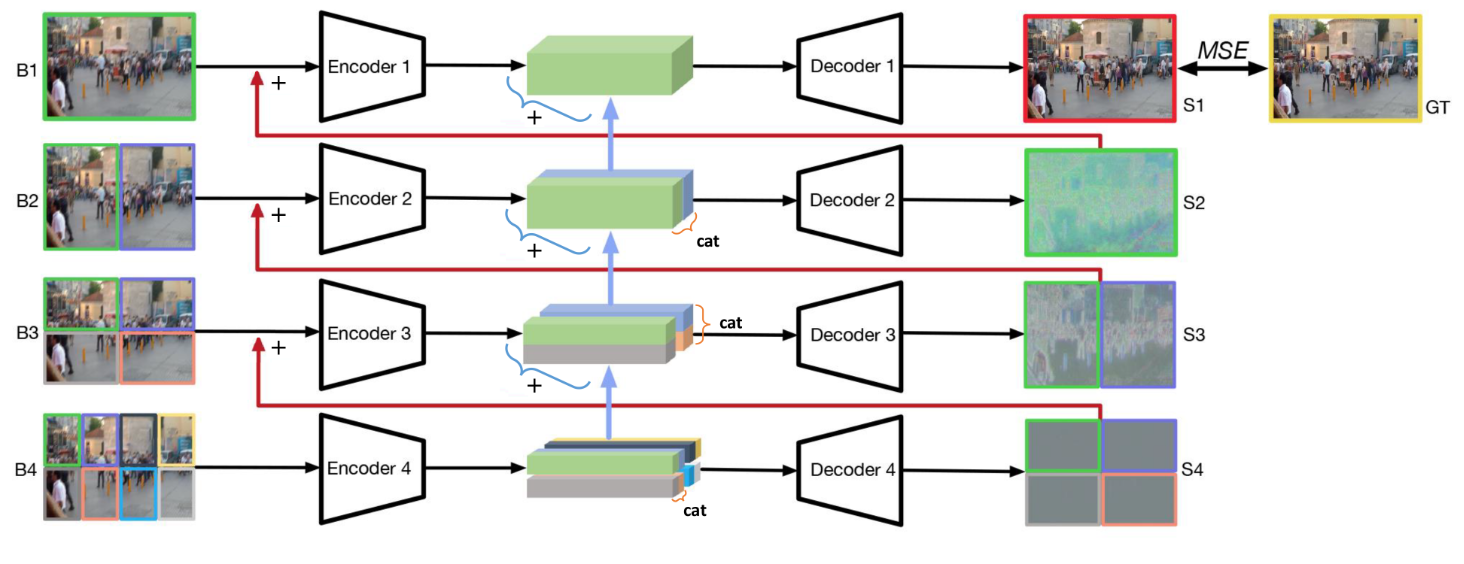
\includegraphics[width=0.8\linewidth]{assets/DMPHN.png}
	\caption{Архитектура DMPHN}
	\label{fig:dmphn}
\end{figure}

\subsection{Модифицированный DMPHN}

Модификации динамической многопатчовой иерархической сети (DMPHN) для устранения размытия изображений включают принятие динамической структуры, в которой фильтрация и рецептивное поле различаются в зависимости от пространственного местоположения и разных входных изображений. Структура сети состоит из трех уровней, каждый из которых имеет кодер и декодер. И кодер, и декодер включают стандартные сверточные слои и остаточные блоки.

На каждом уровне вводится модуль обработки с учетом содержимого, встроенный в каждый остаточный блок. В этом модуле есть две ветви для обработки глобальных и локальных объектов:

\subsubsection*{Глобальная ветвь} В этой ветке используется упрощенный механизм внимания, включающий операцию самоконтроля:

\begin{equation}
	y_{\text{global}} = \text{Softmax}(\text{Conv}(M_{1}) \odot x),
\end{equation}

где \(M_{1}\) — маска пространственного внимания, созданная путем свертки входной карты объектов \(x\).

\subsubsection*{Локальная ветвь} Эта ветвь использует модуль пиксельно-зависимой фильтрации (PDF) для пространственной обработки динамического размытия в движении:

\begin{equation}
	y_{\text{local}} = \sum_{k=1}^{K} \left( V_{j,jk} \cdot W_{c}[jk] \cdot x[j + jk + \Delta jk] \right),
\end{equation}

Здесь \(V_{j,jk}\) представляет собой зависящее от пикселей ядро, сгенерированное PDF, \(W_{c}\) — фиксированный вес, а \(\Delta jk\) — обучаемые смещения.

Механизмы перекрестного внимания реализованы как для взаимодействия кодера-декодера, так и для межуровневого взаимодействия. Перекрестное внимание включает в себя легкий и быстрый механизм внимания:

\begin{equation}
	y_{\text{cross\_attention}} = \text{Softmax}(\text{Conv}(M_{2}) \odot \text{Conv}(M_{1}) \odot x),
\end{equation}

где \(M_{2}\) — еще одна маска пространственного внимания.

Между глобальной и локальной ветвями используется внимательное слияние:

\begin{equation}
	y_{\text{fused}} = M_{\text{fus}} \odot y_{\text{global}} + (1 - M_{\text{fus}}) \odot y_{\text{local }},
\end{equation}

Здесь \(M_{\text{fus}}\) — это маска слияния, созданная на основе исходных входных данных.

Эти модификации направлены на повышение способности DMPHN эффективно справляться с пространственно изменяющимся размытием изображения при выполнении задач устранения размытия изображения \cite{suin2020spatially}.

На рисунке (\ref{fig:modified-dmphn}) представлено, архитектура модифицированный DMPHN: 
\begin{figure}[H]
	\centering
	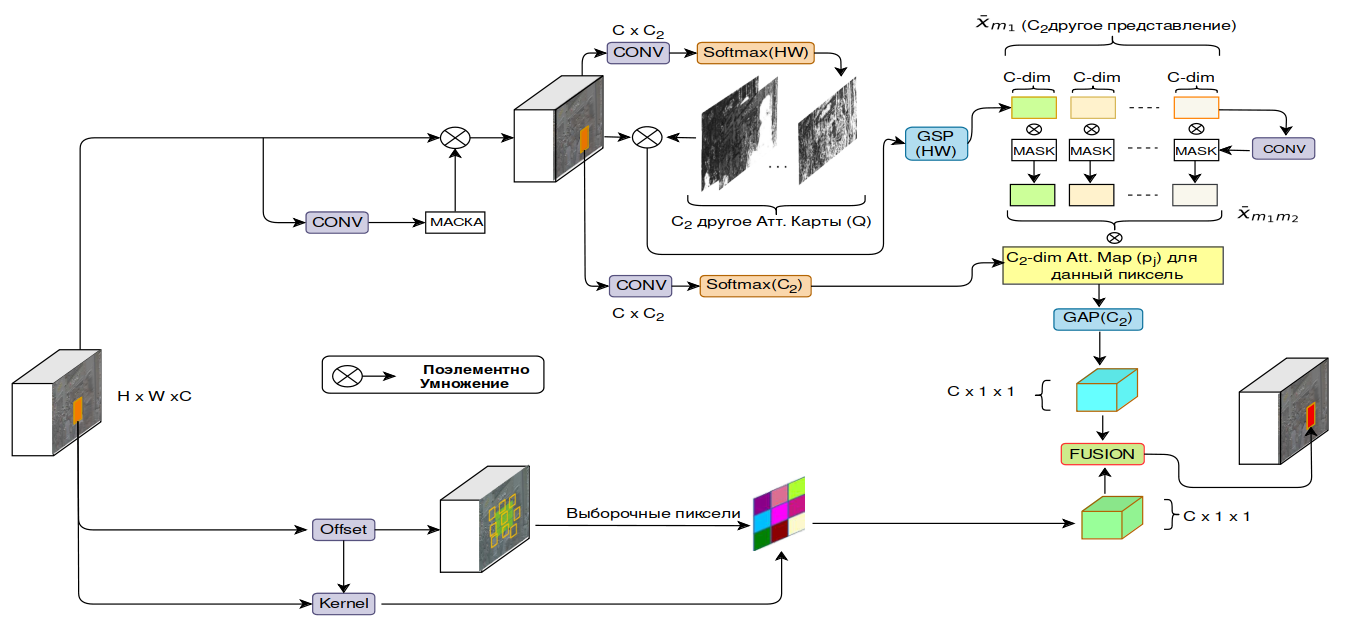
\includegraphics[width=0.7\linewidth]{assets/modified-DMPHN.png}
	\caption{Архитектура модифицированный DMPHN}
	\label{fig:modified-dmphn}
\end{figure}

\subsection{Многоступенчатой прогрессивной реставрации изображения (MPRNet)}

Цель оптимизации предлагаемой сети многоэтапного прогрессивного восстановления (MPRNet) выражается через комплексную функцию потерь, обозначенную как \(L \). Эта функция потерь предназначена для управления сквозной оптимизацией модели на трех ее этапах и формулируется следующим образом:

\begin{equation}
	L = \sum_{S=1}^{3} [L_{char}(X_S, Y) + \lambda L_{edge}(X_S, Y)],
\end{equation}

В этом выражении \( Y \) представляет собой истинное изображение, а \( \lambda \) является параметром, который контролирует относительную важность двух ключевых условий потери: потери Шарбонье \( L_{char} \) и потеря края \( L_{edge} \).

Член потерь Шарбонье \( L_{char} \) определяется как:

\begin{equation}
	L_{char} = \sqrt{(kX_S - Y)^2 + \epsilon^2},
\end{equation}

Этот компонент потерь измеряет попиксельную разницу между предсказанным восстановленным изображением \( X_S \) и основной истиной \( Y \). Включение квадратного корня вместе с небольшой константой \( \epsilon \), установленной эмпирически равной \( 10^{-3} \), обеспечивает численную стабильность в процессе оптимизации.

Член потери края \( L_{edge} \) определяется как:

\begin{equation}
	L_{edge} = \sqrt{(k\Delta(X_S) - \Delta(Y))^2 + \epsilon^2},
\end{equation}

Здесь потеря края фокусируется на количественной оценке разницы в высокочастотных деталях между предсказанными и достоверными изображениями с использованием оператора Лапласа \(\Delta\). Подобно потерям Шарбонье, \( \epsilon \) используется для численной стабильности.

Эти условия потерь в совокупности заставляют модель постепенно совершенствовать восстановление изображений на нескольких этапах. Потеря Шарбонье подчеркивает сохранение содержания изображения, тогда как потеря края отдает приоритет точному восстановлению высокочастотных деталей. Параметр \( \lambda \) позволяет точно настроить баланс между этими двумя целями, способствуя общей эффективности MPRNet в задачах восстановления изображений \cite{zamir2021multi}.

На рисунке (\ref{fig:MPRNet}) представлено, архитектура MPRNet: 
\begin{figure}[H]
	\centering
	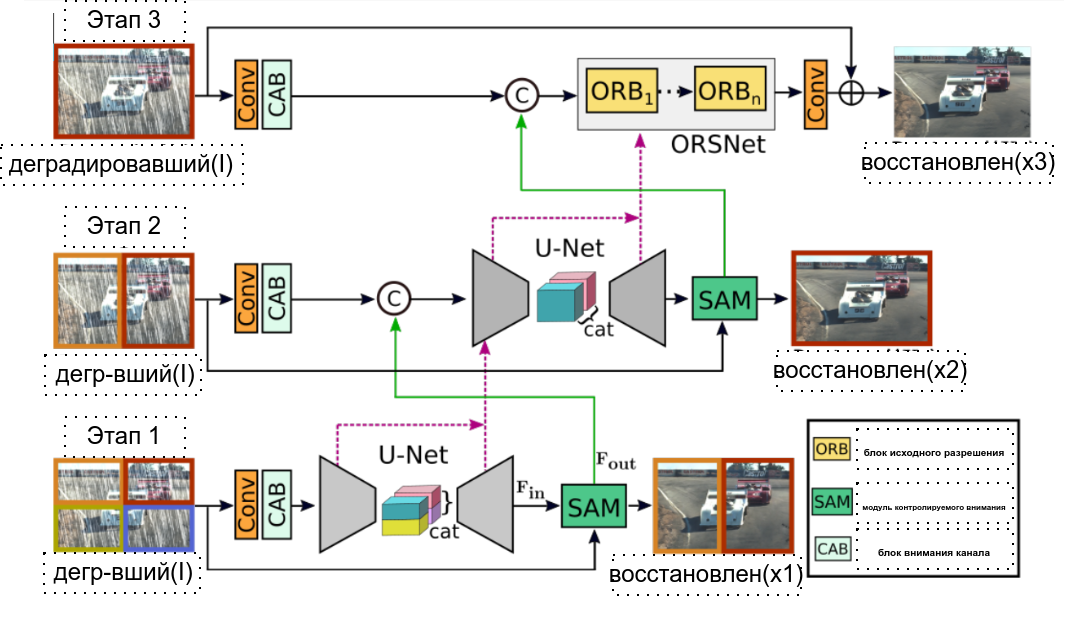
\includegraphics[width=0.7\linewidth]{assets/MPRNet.png}
	\caption{Архитектура MPRNet}
	\label{fig:MPRNet}
\end{figure}

\section{Критерия сравнение методы}

Оценка восстановленных изображений может осуществляться как качественным, так и количественным способом. Количественные подходы обеспечивают более надежный способ оценки качества изображения, используя некоторые показатели, с которыми может согласиться каждый. Рассмотрим часто используемые метрики для работоспособности метода:

\subsection{Среднеквадратическая ошибка (MSE)}

MSE измеряет попиксельную разницу между реальными и восстановленными изображениями:

\begin{equation}\label{eq:mse}
MSE(I, \hat{I}) = \frac{1}{N} \sum_{i=1}^{N} (I_{i} - \hat{I}_{i})^2,
\end{equation}

где \(N\) — общее количество пикселей в рассматриваемом изображении. Эта метрика в основном используется для обучения глубоких сетей, а не для их оценки. Когда он используется для обучения, он аналогичен потере контента, но широко используется в качестве показателя производительности в традиционных подходах, основанных на оптимизации. Чем меньше MSE, тем лучше результат восстановления, то есть восстановленное изображение больше похоже на истинное изображение.

\subsection{Пиковое соотношение сигнал/шум (PSNR)}

PSNR — одна из наиболее широко используемых метрик в приложениях для устранения размытия изображений, и она формулируется как:

\begin{equation}
	PSNR(I, \hat{I}) = 10 \cdot \log_{10} \left( \frac{R^{2}}{MSE(I, \hat{I})} \right),
\end{equation}

где \(R\) — максимально возможное значение пикселя изображения. В большинстве случаев изображения имеют 8-битный формат, поэтому \(R\) принимает значение 255. Качество изображения лучше, если PSNR имеет более высокое значение. Это прямое следствие наличия СКО в знаменателе уравнения (\ref{eq:mse}), что делает две метрики обратно пропорциональными \cite{hore2010image}.

\subsection{Структурная мера сходства (SSIM)}

SSIM также является очень популярным показателем качества изображения. Эта метрика измеряет сходство между двумя изображениями путем сравнения интенсивности пикселей \cite{wang2004image}. Его значения варьируются от нуля до единицы, а более высокое значение указывает на лучшее качество реконструкции. SSIM рассчитывается как:

\begin{equation}
	SSIM(I, \hat{I}) = \frac{{2\mu_I \mu_{\hat{I}} + C_1}}{{\mu_I^2 + \mu_{\hat{I}}^2 + C_1}} \cdot \frac{2\sigma_I \sigma_{\hat{I}} + C_2}{\sigma_I^2 + \sigma_{\hat{I}}^2 + C_2},
\end{equation}

где \(\frac{\mu_{I}}{\sigma_{I}^2}\) и \(\frac{\mu_{\hat{I}}}{\sigma_{\hat{I}}^2}\) - среднее/дисперсия значений пикселей для истинного и восстановленного изображений соответственно. \(C_1\) и \(C_2\) - положительные константы, используемые для стабилизации деления.

Во всех проведенных метриках \(I\) и \(\hat{I}\) обозначают истинное изображение и восстановленное изображение соответственно.

\section{Классификации причислинных методов}

Не смотря на две метрики \(PSNR\) и \(SSIM\), которые часто выделяются для оценки работоспособности метода, можно также рассмотреть следующие критерии для сравнения приведенных методов:
\begin{enumerate}
	\item \(K_{1}\) -- Cпособность метода точно восстанавливать мелкие детали в размытом изображении, обеспечивая четкость и выразительность структурных элементов.
	\item \(K_{2}\) -- Насколько метод способен адаптироваться к разнообразным уровням и типам размытия, подчеркивая его гибкость и эффективность в различных сценариях.
	\item \(K_{3}\) -- Способность метода извлекать и обрабатывать сложные функции изображения, подчеркивая эффективность в работе с разнообразными контекстами и характеристиками изображения.
	\item \(K_{4}\) -- Насколько быстро метод может обучаться, что важно для эффективного внедрения в реальных условиях и ограниченных вычислительных средах.
% Качество восстановления деталей:
% Сохранение общего контента:
% Устойчивость к различным уровням размытия:
% Вычислительная эффективность:
\end{enumerate}

В таблице (\ref{tab:comparison}) проведена классификация приведенных методов для задачи восстановления размытия изображений.

\begin{table}[H]
    \centering
    \caption{Классификация приведенных методов восстановления изображений}
    \label{tab:comparison}
    \begin{tabular}{|p{3cm}|p{3.8cm}|p{4.6cm}|p{3.8cm}|}
        \hline
        \textbf{Критерий сравнения} & \textbf{DMPHN} & \textbf{Модифицированный DMPHN} & \textbf{MPRNet} \\ \hline
        \(K_{1}\) & Стандартное, но эффективное & Улучшенное с учетом структуры & Прогрессивное, высокочастотное \\ \hline
        \(K_{2}\) & Общая устойчивость, но без динамической структуры & Адаптивность к различным уровням и динамическое размытие & Устойчивость и прогрессивное улучшение с каждым этапом \\ \hline
        \(K_{3}\) & Ограниченная адаптивность & Улучшенная с учетом содержимого & Прогрессивное и эффективное \\ \hline
        \(K_{4}\) & Стандартная & Возможно немного медленнее & Оптимизировано для быстрого обучения \\ \hline
    \end{tabular}
\end{table}

\section{Формулировка цели}

Цель данной работы заключается в разработке метода восстановление размытия изображения. Разработанный метод должен обладать следующими характеристиками:

\begin{enumerate}
	\item Принимать на вход размытое изображение.
	\item Применять нейронную сеть для устранения размытия изображения.
	\item Быть способным работать с размытыми изображениями, вид которых неизвестен на входе.
	\item На выходе предоставлять изображение в виде восстановленного изображения.
\end{enumerate}

\section{Формализация задачи}

В данном подразделе рассмотрим формализацию задачи восстановления размытия изображений с применением нейронной сети.

На рисунке (\ref{fig:method-desc-a0}) представлено, формализация задачи восстановление размытие изображение нулевый уровень преобразований: 
\begin{figure}[H]
	\centering
	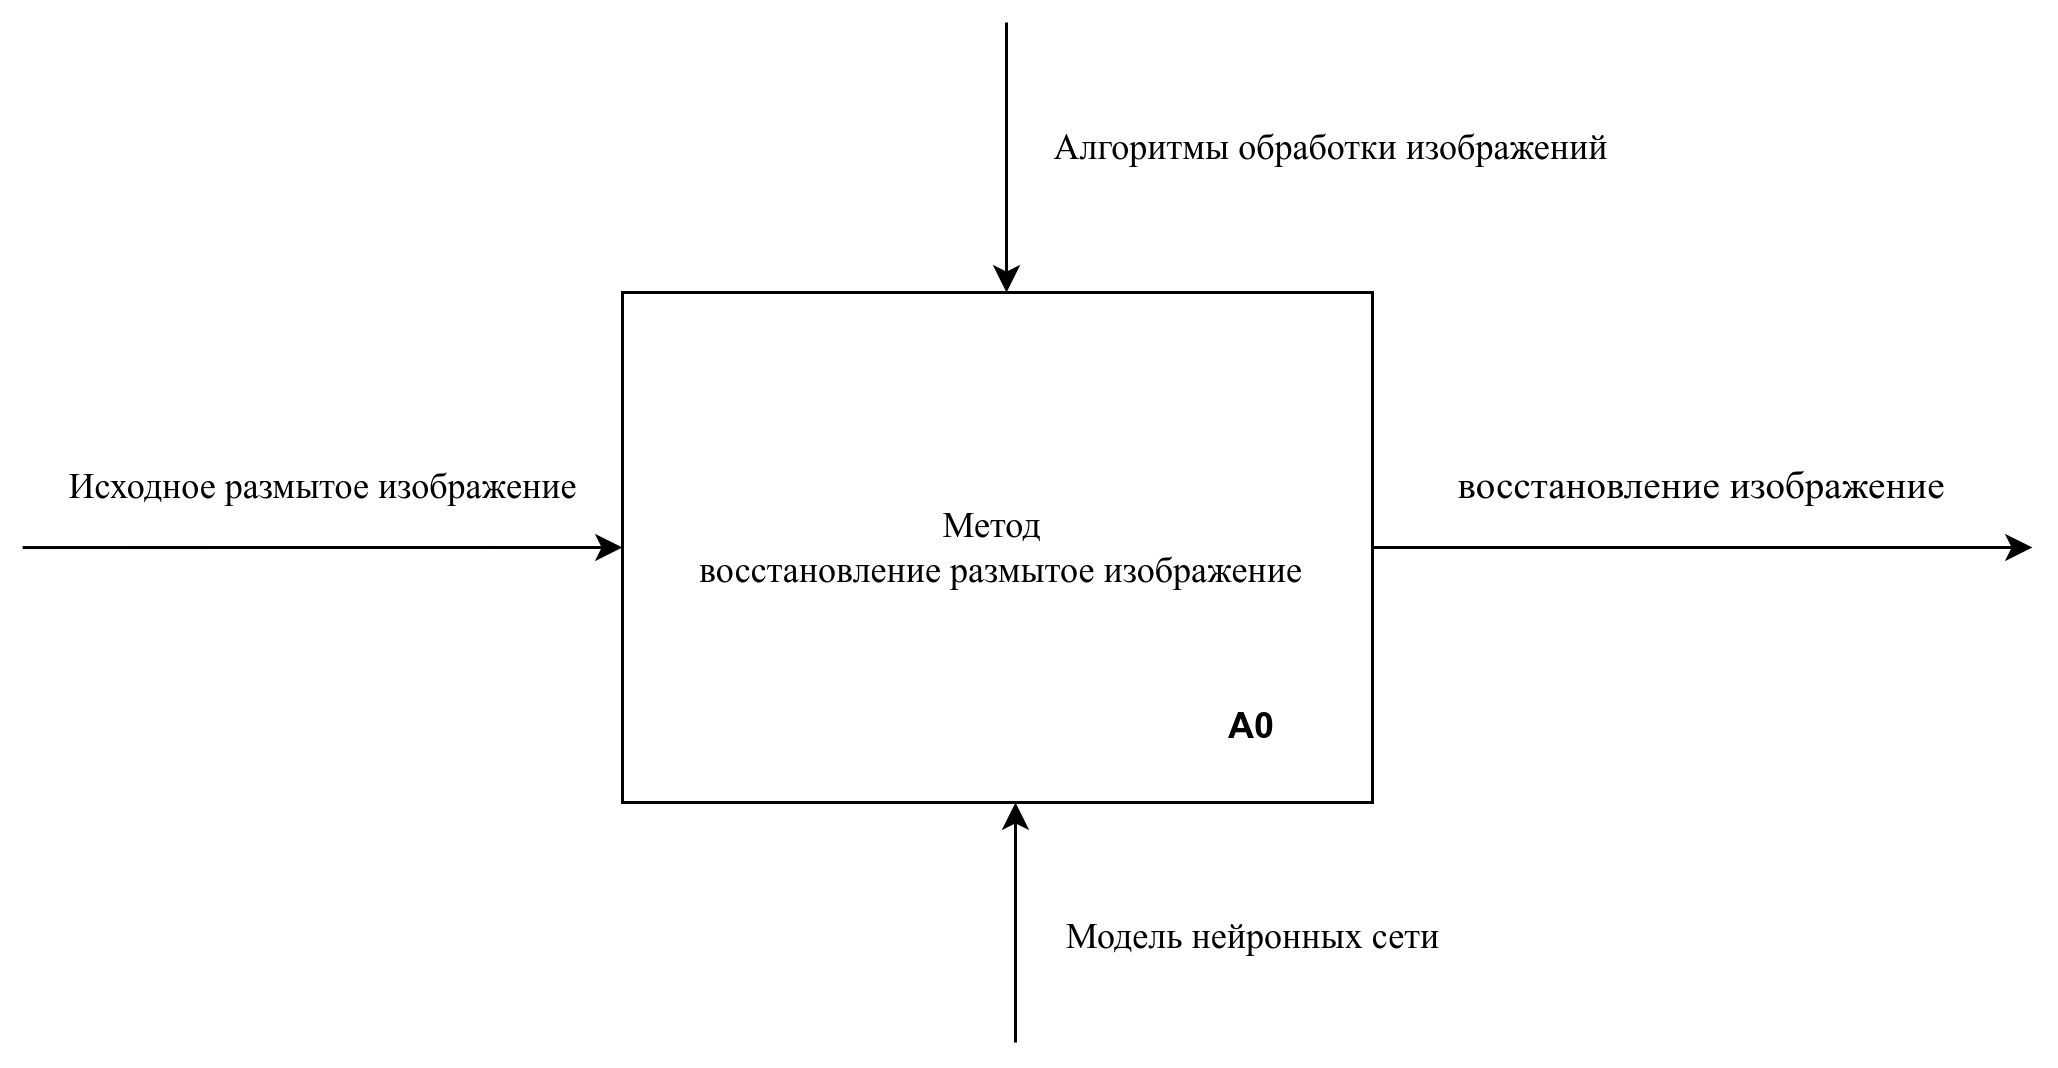
\includegraphics[width=1\linewidth]{assets/idef0-A0.png}
	\caption{Формализация задачи восстановление размытие изображение нулевый уровень преобразований}
	\label{fig:method-desc-a0}
\end{figure}


На рисунке (\ref{fig:method-desc-a0}) представлено, формализация задачи восстановление размытие изображение первый уровень преобразований: 
\begin{figure}[H]
	\centering
	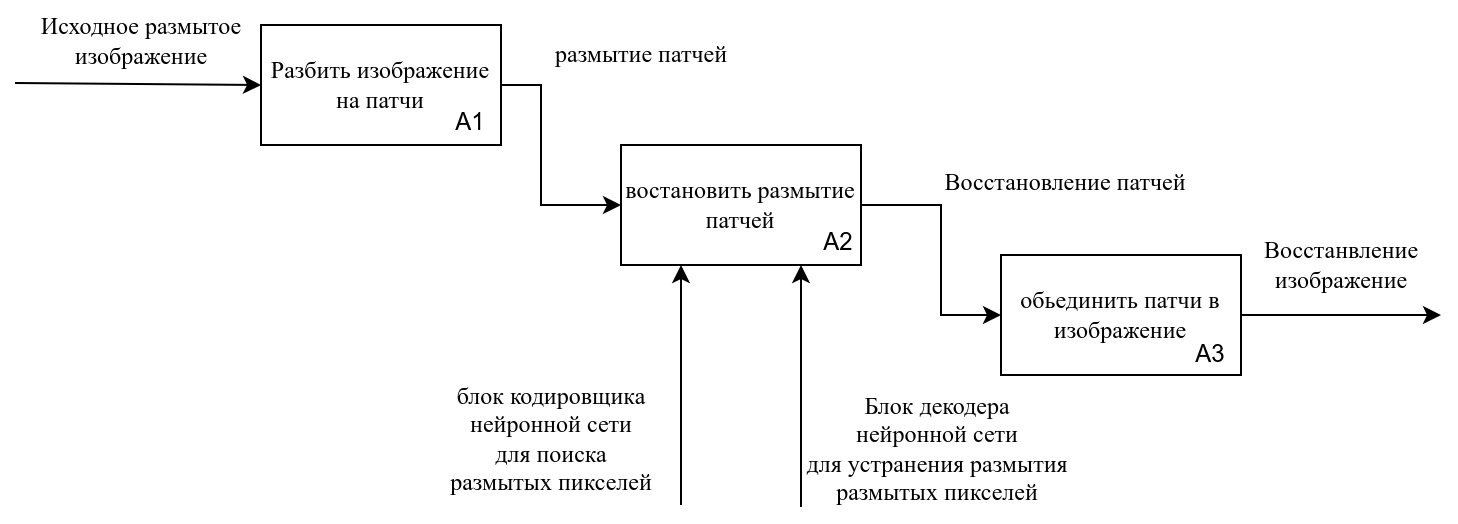
\includegraphics[width=1\linewidth]{assets/idef0-A1.png}
	\caption{Формализация задачи восстановление размытие изображение первый уровень преобразований}
	\label{fig:method-desc-a0}
\end{figure}

\section*{Вывод}

В данном разделе была выполнена постановка цели разработки проекта, проведен анализ предметной области, рассмотрены понятия и существующие методы нейронных сетей для решения поставленной задачи. Осуществлен обзор уже существующих методов, а также установлены критерии сравнения и классификации этих методов. В результате было принято решение разработать метод восстановления размытых изображений с использованием MRPNet в качестве основной архитектуры. Это решение было принято, поскольку данная архитектура эффективно справляется с задачей восстановления размытых изображений.